\documentclass[border = 0.2cm]{standalone}

% import packages
\usepackage{xcolor} % color packages
%\usepackage{pgfkeys} % pgf-keys package
\usepackage{tikz} % package for drawing
\usetikzlibrary{arrows, snakes, backgrounds, petri} % tikz's libraries 

% define styles for shapes of node, arrows and label
\tikzstyle{place} = [circle, thick, minimum size = 6mm, draw = blue!75, fill = blue!20]
\tikzstyle{transition} = [rectangle, thick, minimum size = 6mm, draw = black!75, fill = black!20]
\tikzstyle{pre} = [<-, shorten <= 1pt, >= stealth, semithick]
\tikzstyle{post} = [->, shorten >= 1pt, >= stealth, semithick]
\tikzstyle{red place} = [place, draw = red!75, fill = red!20]
\tikzstyle{every label} = [red]

\begin{document}
    % begin of picture
    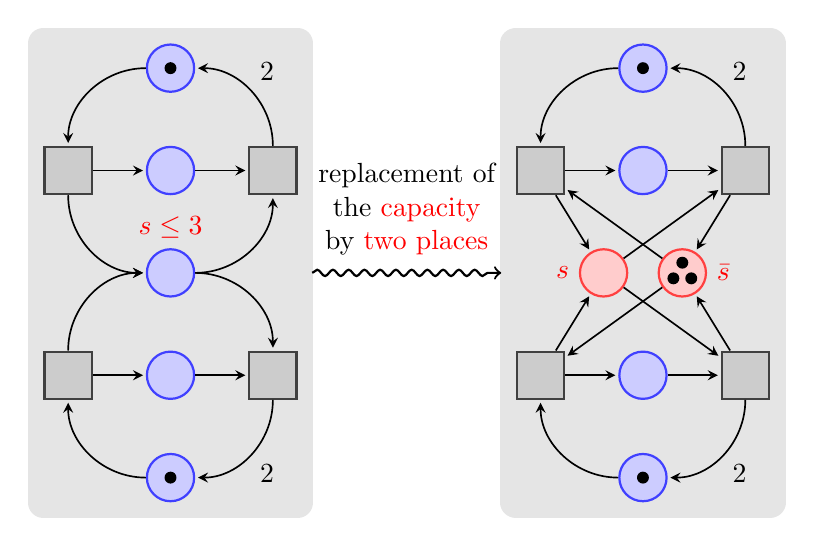
\begin{tikzpicture}[node distance = 1.3cm, >= stealth, bend angle = 45, auto]
        % draw first net (left net)
        % draw nodes
        \node[place, tokens=1] (w1) {};
        \node[place] (c1) [below of = w1] {};
        \node[place] (s) [below of = c1, label = above:$s\le 3$] {};
        \node[place] (c2) [below of = s] {};
        \node[place, tokens=1] (w2) [below of = c2] {};
        % draw arrows and add label on arrows
        \node[transition] (e1) [left of = c1] {}
            edge [pre, bend left] (w1)
            edge [post, bend right] (s)
            edge [post] (c1);
        \node[transition] (e2) [left of = c2] {}
            edge [pre, bend right] (w2)
            edge [post, bend left] (s)
            edge [post] (c2);
        \node[transition] (l1) [right of = c1] {}
            edge [pre] (c1)
            edge [pre, bend left] (s)
            edge [post, bend right] node[swap] {2} (w1);
        \node[transition] (l2) [right of = c2] {}
            edge [pre] (c2)
            edge [pre, bend right] (s)
            edge [post, bend left] node {2} (w2);
        
        % draw second net 
        \begin{scope}[xshift = 6cm]
            % draw nodes
            \node[place, tokens=1] (w1') {};
            \node[place] (c1') [below of = w1'] {};
            \node[red place] (s1') [below of = c1', xshift = -5mm] [label = left:$s$] {};
            \node[red place, tokens=3] (s2') [below of = c1', xshift = 5mm] [label = right:$\bar{s}$] {};
            \node[place] (c2') [below of = s1', xshift = 5mm] {};
            \node[place, tokens=1] (w2') [below of = c2'] {};
            % draw arrows and add label on arrows
            \node[transition] (e1') [left of = c1'] {}
                edge [pre, bend left] (w1')
                edge [post] (s1')
                edge [pre] (s2')
                edge [post] (c1');
            \node[transition] (e2') [left of = c2'] {}
                edge [pre, bend right] (w2')
                edge [post] (s1')
                edge [pre] (s2')
                edge [post] (c2');
            \node[transition] (l1') [right of = c1'] {}
                edge [pre] (c1')
                edge [pre] (s1')
                edge [post] (s2')
                edge [post, bend right] node[swap] {2} (w1');
            \node[transition] (l2') [right of = c2'] {}
                edge [pre] (c2')
                edge [pre] (s1')
                edge [post] (s2')
                edge [post, bend left] node {2} (w2');
        \end{scope}
        
        % draw snake
        \draw[-to, thick, snake = snake, segment amplitude = .4mm, segment length = 2mm, line after snake = 1mm]
        ([xshift = 5mm]s -| l1) -- ([xshift = -5mm]s1' -| e1')
        node [above = 1mm, midway, text width = 3cm, text centered]
        {replacement of the \textcolor{red}{capacity} by \textcolor{red}{two places}};
        
        % draw background
        \begin{pgfonlayer}{background}
            \filldraw [line width = 4mm, join = round, black!10]
            (w1.north -| l1.east) rectangle (w2.south -| e2.west)
            (w1'.north -| l1'.east) rectangle (w2'.south -| e1'.west);
        \end{pgfonlayer}
    \end{tikzpicture}
    % end of picture
\end{document}